% 2001 年春季京蒙皖理卷第 19 题：斜线与三棱锥空间关系
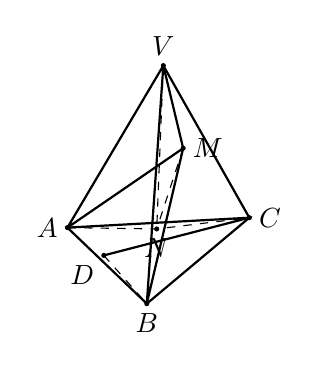
\begin{tikzpicture}[>=stealth, scale=0.84]
  \coordinate (A) at (0,0);
  \coordinate (B) at (1.2,-1.15);
  \coordinate (C) at (2.75,0.15);
  \coordinate (D) at (0.55,-0.42);
  \coordinate (N) at (1.35,-0.02);
  \coordinate (M) at (1.75,1.2);
  \coordinate (V) at (1.45,2.45);

  \draw[thick] (A)--(B)--(C)--cycle;
  \draw[thick] (C)--(D);
  \draw[dashed] (D)--(B) (A)--(N)--(C);
  \draw[thick] (V)--(C) (V)--(A) (V)--(B) (M)--(A) (M)--(B);
  \draw[dashed] (V)--(N) (M)--(N);
  \draw[thick] (V)--(M);

  \fill (A) circle (1.1pt) node[left] {$A$};
  \fill (B) circle (1.1pt) node[below] {$B$};
  \fill (C) circle (1.1pt) node[right] {$C$};
  \fill (D) circle (1.1pt) node[below left] {$D$};
  \fill (N) circle (1.1pt) node[below] {$N$};
  \fill (M) circle (1.1pt) node[right] {$M$};
  \fill (V) circle (1.1pt) node[above] {$V$};
\end{tikzpicture}
